\documentclass[twoside,twocolumn]{article}
\usepackage{blindtext}
\usepackage{graphicx}
\usepackage[sc]{mathpazo}
\usepackage[T1]{fontenc}
\linespread{1.05} 
\usepackage{microtype}
\usepackage[english, spanish]{babel}
\usepackage[hmarginratio=1:1,top=32mm,columnsep=20pt]{geometry}
\usepackage[hang, small,labelfont=bf,up,textfont=it,up]{caption}
\usepackage{booktabs}
\usepackage{lettrine}
\usepackage{enumitem}
\setlist[itemize]{noitemsep}
\usepackage{abstract}
\renewcommand{\abstractnamefont}{\normalfont\bfseries} 
\renewcommand{\abstracttextfont}{\normalfont\small\itshape} 
\usepackage{titlesec}
\renewcommand\thesection{\Roman{section}} % 
\renewcommand\thesubsubsection{\roman{subsubsection}} 
\titleformat{\section}[block]{\large\scshape\centering}{\thesection.}{1em}{}
\titleformat{\subsubsection}[block]{\large}{\thesubsubsection.}{1em}{}
\usepackage{fancyhdr} 
\pagestyle{fancy} % All pages have headers and footers
\fancyhead{} % Blank out the default header
\fancyfoot{} % Blank out the default footer
\fancyhead[L]{Comparativa de metodologías de elaboración de DataWarehouses vs DataLakes} % Custom header text
\fancyhead[R]{Mayo 2021} % Custom header text
\fancyfoot[RO,LE]{\thepage} % Custom footer text
\usepackage{titling}
\usepackage{hyperref}

%----------------------------------------------------------------------------------------
%	TILULOS
%----------------------------------------------------------------------------------------

\setlength{\droptitle}{-4\baselineskip}

\pretitle{\begin{center}\Huge\bfseries}
\posttitle{\end{center}} 
\title{Comparativa de metodologías de elaboración de DataWarehouses vs DataLakes}
\author{Jose Arias, Jose Gutierrez, Posi Vargas, Rodrigo Yanqui, Roby Zuñiga}
\date{\today} 
\renewcommand{\maketitlehookd}{
\selectlanguage{spanish}
\begin{abstract}
\noindent Cada vez es más común que las empresas traten de buscar soluciones al almacenamiento de grandes volúmenes de datos recurriendo a la tecnología Big Data. En este contexto, para gestionar toda esta información los profesionales pueden optar por dos sistemas, Data Lake o Data Warehouse. A veces su elección genera dudas así que vamos a ver en detalle en qué consiste cada uno de ellos, así como sus principales diferencias para que cada empresa pueda tomar la mejor elección para sus proyectos.
\end{abstract}
\selectlanguage{english}
\begin{abstract}
\noindent It is increasingly common for companies to try to look for solutions to the storage of large volumes of data by resorting to Big Data technology. In this context, to manage all this information, professionals can opt for two systems, Data Lake or Data Warehouse. Sometimes your choice generates doubts so let's see in detail what each of them consists of, as well as their main differences so that each company can take the best choice for their projects.
\end{abstract}
}

%----------------------------------------------------------------------------------------

\begin{document}

% Print the title
\maketitle

%----------------------------------------------------------------------------------------
%	INTRODUCCION
%----------------------------------------------------------------------------------------

\section{Introduccion}
\lettrine[nindent=0em,lines=3]{I}nternet y las nuevas tecnologías han provocado el acceso y el almacenamiento desmesurado de información de los clientes y potenciales.\\[0.1in]
Las empresas son cada vez más conscientes de la importancia que tienen esos datos para conocer mejor a los usuarios y así poder ofrecerles aquello que realmente piden, y no lo que nosotros pensamos que necesitan. Esto es lo que se llama, aplicar estrategias customer centric.\\[0.1in]
Para ello se necesita gestionar altos volúmenes de datos, tanto en tiempo real como organizados. Para ello, no hay nada mejor que un Data Warehouse o un Data Lake.

%----------------------------------------------------------------------------------------
%	DESARROLLO
%----------------------------------------------------------------------------------------

\section{Desarrollo}

\subsection{¿Qué es el Data Warehouse?}
\noindent Data Warehouse es una combinación de tecnologías y componentes para el uso estratégico de datos. Recopila y gestiona datos de diversas fuentes para proporcionar información empresarial significativa. Es el almacenamiento electrónico de una gran cantidad de información diseñada para consultas y análisis en lugar de procesamiento de transacciones. Es un proceso de transformación de datos en información.\\[0.1in]
Las funciones importantes que se deben realizar son:
\begin{itemize}
    \item Extracción de datos.
    \item Limpieza de datos.
    \item Transformación de datos.
    \item Carga y actualización de datos.    
\end{itemize}
\begin{center}
    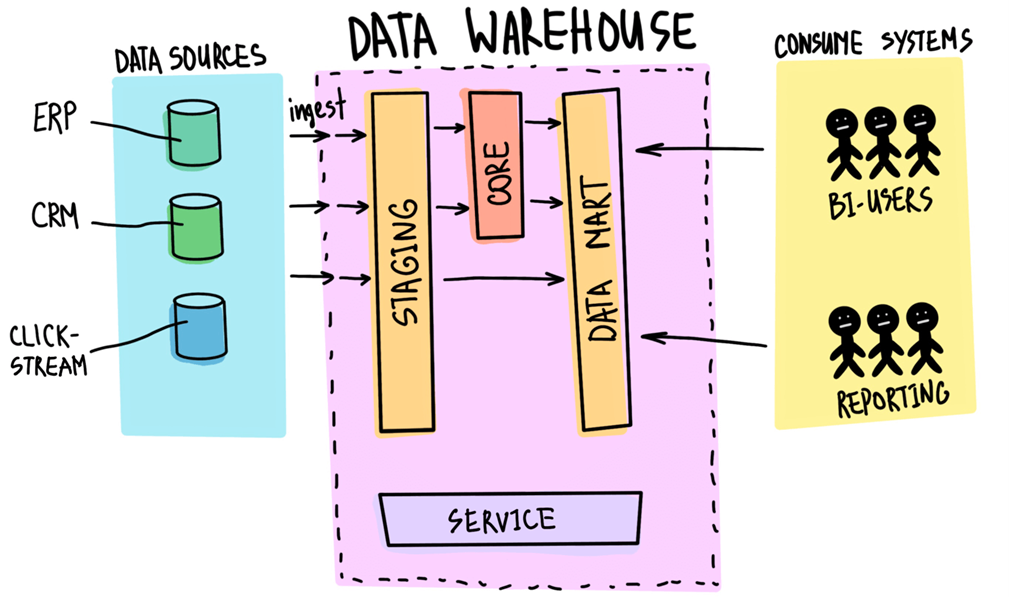
\includegraphics[width=7cm]{./img/img1.png}
\end{center}

\textbf{\large Ventajas de un Data Warehouse}
\begin{itemize}
    \item La data está lista para ser usada.
    \item Buena performance en el acceso a los datos.
    \item La mayoría de los usuarios de una empresa son operacionales, data warehouse es ideal para ellos.
    \item Es muy adecuado para generar reportes y métricas.
\end{itemize}

\textbf{\large Desventajas de un Data Warehouse}
\begin{itemize}
    \item Mayores costos de almacenamiento, lo que implica pensar bien qué data es realmente necesaria.
    \item No es flexible a cambios.
    \item Demanda inversión de tiempo antes del almacenamiento para decidir esquemas, formatos y casos de uso.
\end{itemize}

\subsection{¿Qué es Data Lake?}
\noindent Un Data Lake es un repositorio de almacenamiento que puede almacenar una gran cantidad de datos estructurados, semiestructurados y no estructurados. Es un lugar para almacenar todo tipo de datos en su formato nativo sin límites fijos en el tamaño de la cuenta o el archivo. Ofrece una gran cantidad de datos para un mayor rendimiento analítico e integración nativa.\\[0.1in]
Data Lake es como un gran contenedor que es muy similar a los lagos y ríos reales. Al igual que en un lago, entran múltiples afluentes. De manera similar, un lago de datos tiene datos estructurados, datos no estructurados, máquina a máquina, registros que fluyen en tiempo real.
\begin{center}
    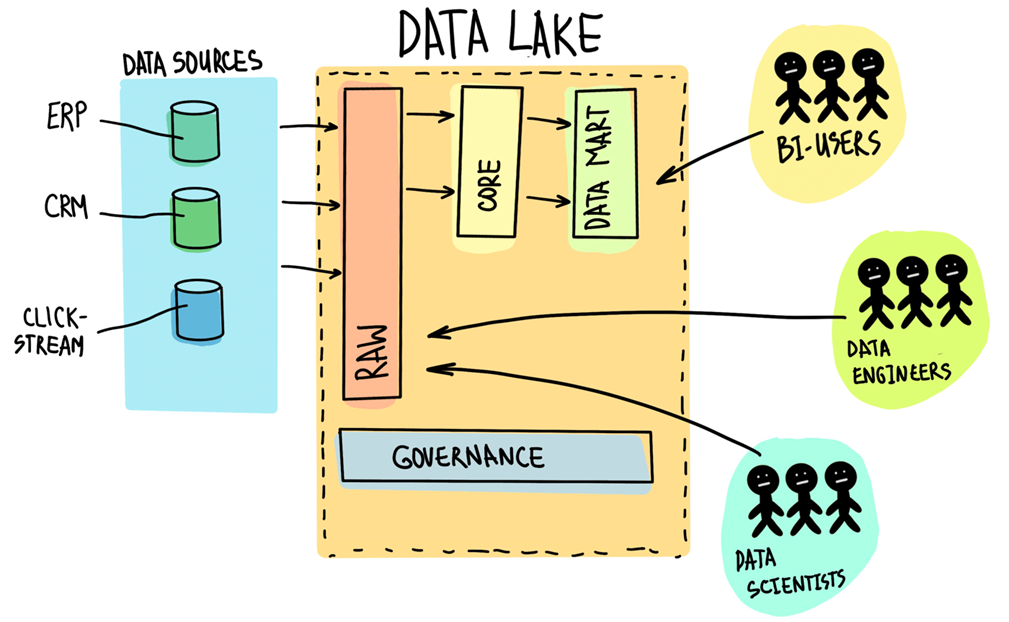
\includegraphics[width=7cm]{./img/img2.png}
\end{center}

\textbf{\large Ventajas de un Data Lake}
\begin{itemize}
    \item No hay necesidad de descartar datos.
    \item Puede nutrir a diversos usuarios de una empresa.
    \item Se adapta fácilmente a los cambios.
    \item Al poder integrarse tipos de datos muy distintos, se puede realizar todo tipo de análisis.
    \item Permite fácilmente agregar nueva data.
\end{itemize}

\textbf{\large Desventajas de un Data Lake}
\begin{itemize}
    \item No está pensado para acceder a los datos de manera performante.
    \item Cada vez que se requieren datos, hay que transformarlos y curarlos para el uso que se les quiera dar.
    \item Demanda invertir en generar estándares de buenas prácticas a nivel organizacional.
\end{itemize}

\subsection{Diferencia clave entre Data Lake y Data Warehouse}
\begin{center}
    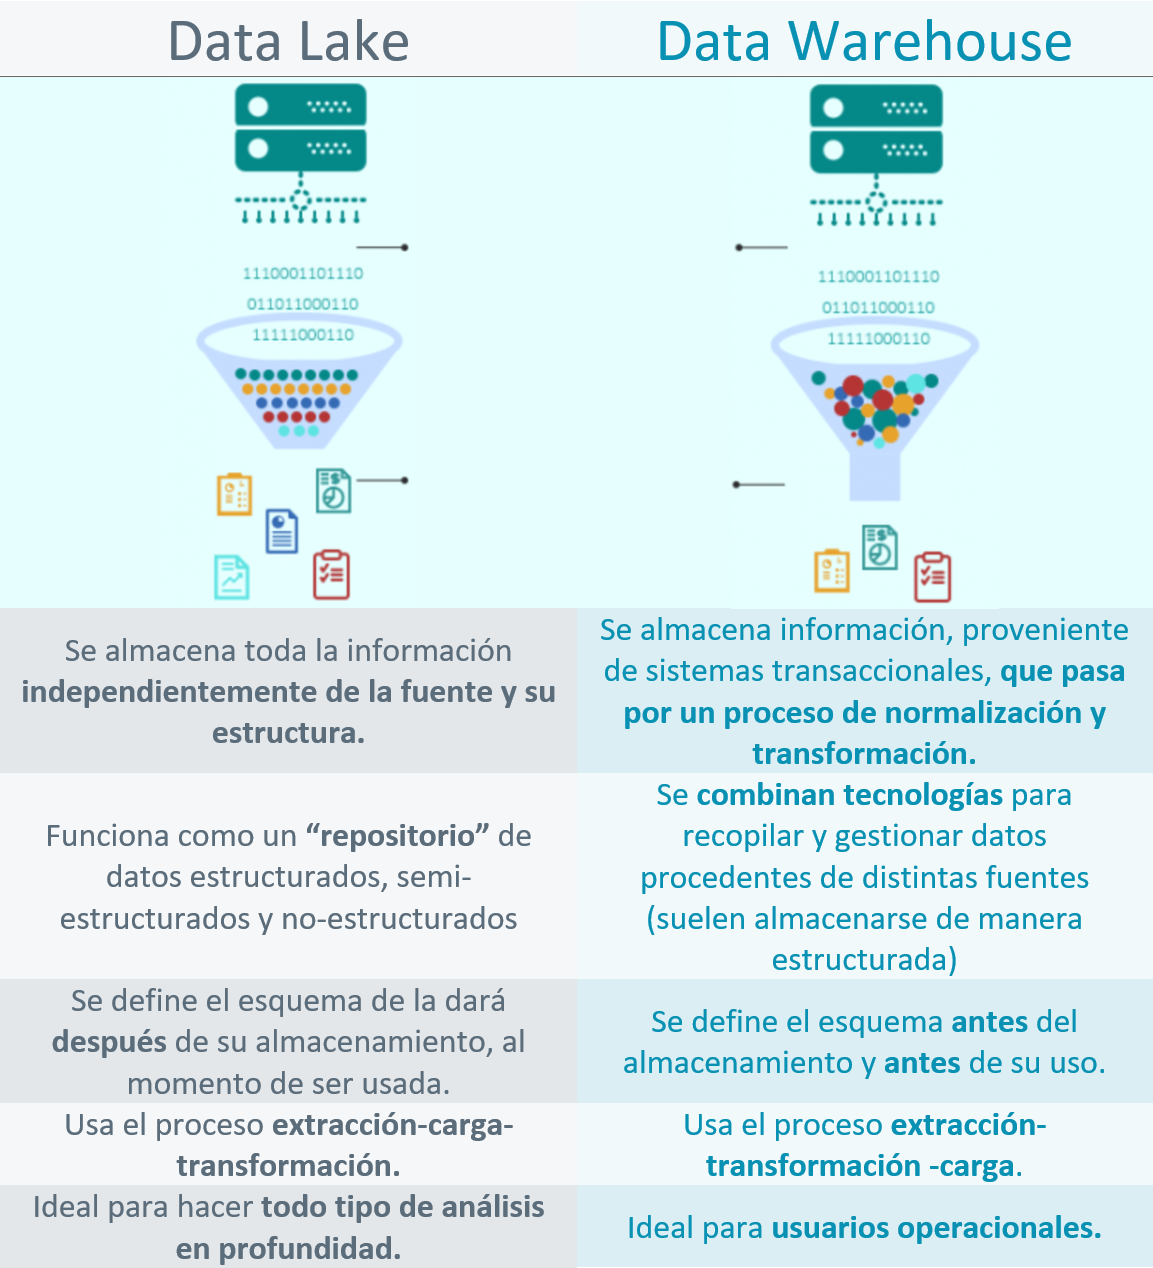
\includegraphics[width=7cm]{./img/img3.png}
\end{center}

\subsection{Comparación de Metodologías de Elaboración}
\noindent Una de las diferencias que marcan la comparación entre Data Lake vs Data Warehouse es que, este último, por lo general, sigue una metodología como las definidas por Inmon y Kimball, a diferencia de Data Lakes.
\paragraph{\Large Metodologías de Data Warehouse \\[0.1in]}
Al diseñar una solución de Data Warehouse, las organizaciones se topan con distintas metodologías y enfoques a seguir, las cuales se deberán evaluar para seleccionar la que mejor se adapte a los requisitos del proyecto.\\[0.1in]
Las siguientes metodologías fueron diseñadas por Ralph Kimball, Bill Inmon y Dan Linsted correspondientemente.\\[0.1in]

\noindent\textbf{\large 1. Dimensional (BUTTON UP / ASCENDENTE)}\\[0.1in]
La metodología dimensional o metodología de Ralph Kimball, mantiene un diseño ascendente por lo que los Data Marts son los primeros en crearse y después se integran al Data Warehouse creando un almacenamiento más completo.\\[0.1in]
Busca que el almacenamiento de datos de los usuarios se ejecute de la forma más rápida posible. Según Kimball, un almacenamiento de datos es la copia de los datos transaccionales específicamente estructurados para consultas analíticas e informes con el fin de apoyar la toma de decisiones. Con su metodología al crear primero los Data Marts se proporcionan capacidades analíticas y de informes para procesos específicos de negocio y funcionales.\\[0.1in]
\textbf{Principales Diferenciadores}
\begin{itemize}
    \item Para mantener el Data Warehouse solo se requiere de un equipo pequeño de desarrolladores y arquitectos de datos.
    \item Brinda buena funcionalidad para las métricas en cuanto al departamento y el seguimiento de KPI, al orientar los Data Marts a informes en cuanto a procesos de departamento o de negocios.
\end{itemize}
\begin{center}
    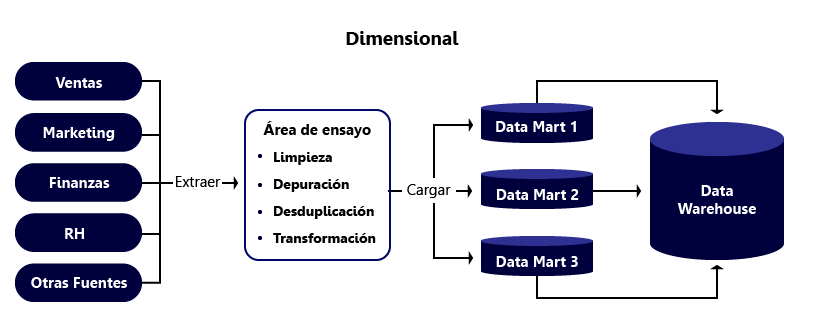
\includegraphics[width=7cm]{./img/img4.png}
\end{center}
La metodología de Kimball propone crear una matriz de negocio que contenga los elementos comunes que son utilizados por los Data Marts, como conformed-shared dimension, measures, etc., teniendo esta información, el usuario puede desarrollar soluciones que apoyen el análisis a través de los procesos de negocio para la venta cruzada.\\[0.1in]

\noindent\textbf{\large 2. Relacional (TOP DOWN / DESCENDENTE)}\\[0.1in]
La metodología relacional de Bill Inmon muestra un diseño descendente, donde se construye primero el Data Warehouse y por consiguiente los Data Marts. Ubicando el DW en el centro de la información corporativa lo que asegura un marco lógico en los datos.\\[0.1in]
Crear una estructura de entidades procurando que no se repitan datos.  Este modelo crea una única fuente de verdad para todo el negocio. La carga de datos se vuelve menos compleja debido a la estructura normalizada del modelo. Sin embargo, el uso de esta disposición para realizar consultas es complicado, ya que incluye gran cantidad de tablas y vínculos.\\[0.1in]
Este modelo propone la construcción de Data Marts por separado para cada departamento. Todos los datos que entran en el Data Warehouse están integrados. Para garantizar la integridad y la coherencia en toda la empresa, el Data Warehouse actúa como un único origen de datos para varios Data Marts.\\[0.1in]
\textbf{Principales Ventajas}
\begin{itemize}
    \item El Data Warehouse proporciona una única versión de la verdad, al ser el único origen de datos para los Data Marts.
    \item Es para los usuarios comprender más fácilmente los procesos empresariales, ya que el modelo lógico representa entidades empresariales detalladas.
    \item Resulta más fácil y menos propenso al fracaso el proceso de ETL, puesto que en la actualización de los datos las anomalías se evitan al contar con una redundancia muy baja.
\end{itemize}
\begin{center}
    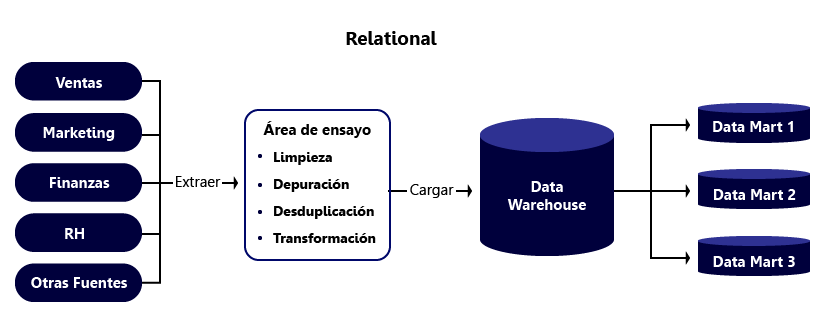
\includegraphics[width=7cm]{./img/img5.png}
\end{center}

\noindent\textbf{\large 3. Data Vault}\\[0.1in]
Es una metodología de seguimiento histórico orientado a los detalles y conjunto de tablas normalizadas vinculadas de forma única que admiten una o más áreas funcionales de negocios. Es un modelo de datos que está diseñado específicamente para cumplir las necesidades de uno o varios Data Warehouse empresariales.\\[0.1in]
\textbf{Principales Ventajas}
\begin{itemize}
    \item Diseñado especialmente para almacenar registros. Hace que el proceso de registro de datos sea más sencillo.
    \item Con esta metodología, es más fácil agregar un nuevo origen de datos sin modificar el ya existente.
    \item Automatiza fácilmente los procesos ETL.
\end{itemize}
\textbf{Arquitectura de Data Vault}\\[0.1in]
Data Vault contiene tres tablas básicas:
\begin{itemize}
    \item Hub
    \item Links
    \item Satélites
\end{itemize}
\begin{center}
    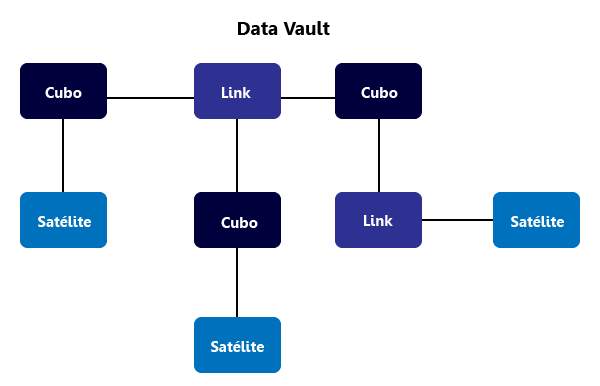
\includegraphics[width=7cm]{./img/img6.png}
\end{center}

%----------------------------------------------------------------------------------------
%	CONCLUSIONES
%----------------------------------------------------------------------------------------

\section{Conclusiones}
\noindent Tanto los Data Warehouses como los Data Lakes están destinados a convivir en las empresas que deseen basar sus decisiones en datos. Como se puede entender, ambos son complementarios, no sustitutivos, pudiendo ayudar a cualquier negocio a conocer mejor el mercado y el consumidor, de cara a poder realizar estrategias basadas en el conocimiento de estos, con comunicaciones cada vez más personalizadas, es decir, ser más customer centric.
\begin{center}
    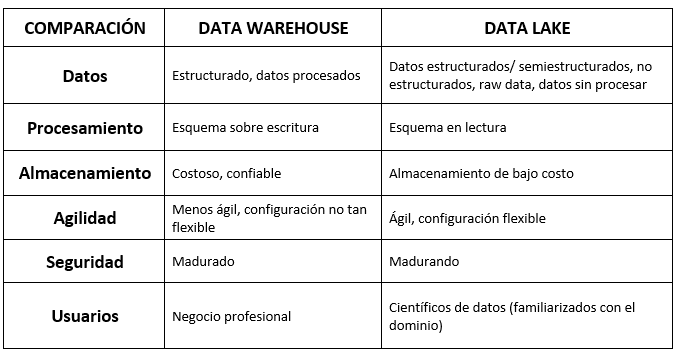
\includegraphics[width=7cm]{./img/img7.png}
\end{center}

%----------------------------------------------------------------------------------------
%	RECOMENDACIONES
%----------------------------------------------------------------------------------------

\section{Recomendaciones}
\noindent El data warehouse responde a necesidades más maduras, cuando ya sabemos qué data es la más importante y qué tipo de trabajo vamos a hacer con ella.\\[0.1in]
Por el otro lado, los data lakes son alternativas más ágiles, baratas y flexibles: atributos muy deseables para empresas jóvenes, como puede ser tu startup.\\[0.1in]
Los data lakes pueden ser especialmente efectivos cuando no sabemos bien qué queremos hacer con toda nuestra data, pero sabemos que la información es potencialmente valiosa.

%----------------------------------------------------------------------------------------
%	BIBLIOGRAFIA
%----------------------------------------------------------------------------------------

\begin{thebibliography}{99} 
    \bibitem{}
    AWS (2020). Data lake on AWS. Recuperado de 
    \\\texttt{https://cutt.ly/4nod8Lm}
    \bibitem{}
    AWS (2019). Data Lake Foundation on the AWS Cloud. Recuperado de 
    \\\texttt{https://cutt.ly/lnod5w8}
    \bibitem{}
    Data Kitchen (2020). Agile Data Lake and Warehouse. Recuperado de 
    \\\texttt{https://cutt.ly/Tnod6Bj}
    \bibitem{}
    Google Cloud (2020). Cloud Storage as a data lake. Recuperado de 
    \\\texttt{https://cutt.ly/RnofwG5}
    \bibitem{}
    IKimball, R. (2016). The Kimball Group Reader: Relentlessly Practical Tools for Data Warehousing and Business Intelligence Remastered Collection. Recuperado de 
    \\\texttt{https://cutt.ly/Jnofruq}
\end{thebibliography}
%----------------------------------------------------------------------------------------
\end{document}